%Art des Dokuments%
\documentclass[a4paper, 11pt]{article}

%Packete
\usepackage{ifxetex,ifluatex}
\usepackage{etoolbox}
\usepackage[svgnames]{xcolor}
\usepackage{amssymb}
\usepackage{tikz}
\usepackage{tcolorbox}
\usepackage{framed}
\usepackage[]{algorithm2e}

% conditional for xetex or luatex
\newif\ifxetexorluatex
\ifxetex
\xetexorluatextrue
\else
\ifluatex
\xetexorluatextrue
\else
\xetexorluatexfalse
\fi
\fi
%
\ifxetexorluatex
\usepackage{fontspec}
\usepackage{libertine} % or use \setmainfont to choose any font on your system
\newfontfamily\quotefont[Ligatures=TeX]{Linux Libertine O} % selects Libertine as the quote font
\else
\usepackage[utf8]{inputenc}
\usepackage[T1]{fontenc}
\usepackage{libertine} % or any other font package
\newcommand*\quotefont{\fontfamily{LinuxLibertineT-LF}} % selects Libertine as the quote font
\fi

\newcommand*\quotesize{60} % if quote size changes, need a way to make shifts relative
% Make commands for the quotes
\newcommand*{\openquote}
{\tikz[remember picture,overlay,xshift=-4ex,yshift=-2.5ex]
	\node (OQ) {\quotefont\fontsize{\quotesize}{\quotesize}\selectfont``};\kern0pt}

\newcommand*{\closequote}[1]
{\tikz[remember picture,overlay,xshift=4ex,yshift={#1}]
	\node (CQ) {\quotefont\fontsize{\quotesize}{\quotesize}\selectfont''};}

% select a colour for the shading
\colorlet{shadecolor}{Azure}

\newcommand*\shadedauthorformat{\emph} % define format for the author argument

% Now a command to allow left, right and centre alignment of the author
\newcommand*\authoralign[1]{%
	\if#1l
	\def\authorfill{}\def\quotefill{\hfill}
	\else
	\if#1r
	\def\authorfill{\hfill}\def\quotefill{}
	\else
	\if#1c
	\gdef\authorfill{\hfill}\def\quotefill{\hfill}
	\else\typeout{Invalid option}
	\fi
	\fi
	\fi}
% wrap everything in its own environment which takes one argument (author) and one optional argument
% specifying the alignment [l, r or c]
%
\newenvironment{shadequote}[2][l]%
{\authoralign{#1}
	\ifblank{#2}
	{\def\shadequoteauthor{}\def\yshift{-2ex}\def\quotefill{\hfill}}
	{\def\shadequoteauthor{\par\authorfill\shadedauthorformat{#2}}\def\yshift{2ex}}
	\begin{snugshade}\begin{quote}\openquote}
		{\shadequoteauthor\quotefill\closequote{\yshift}\end{quote}\end{snugshade}}


\usepackage[ngerman]{babel}
%\usepackage[latin1]{inputenc}
\usepackage{color}
\usepackage[a4paper, lmargin={4cm}, rmargin={2cm}, tmargin={2,5cm}, bmargin={2,5cm}]{geometry}
\usepackage{graphicx}
\usepackage{setspace}
\usepackage{framed}
\usepackage{url}
\usepackage{eurosym}
\usepackage{acronym}
\usepackage{listings}
\usepackage{color}
\usepackage{longtable}
\usepackage{courier}
\usepackage[multiple]{footmisc}
\usepackage{selinput}
\usepackage{array}
\usepackage{multirow}
\usepackage{longtable}
\usepackage{amssymb}
\usepackage{booktabs}
\usepackage[framemethod=TikZ]{mdframed}
%mdframed Einstellungen%
\newenvironment{theo}[2][]{%
	\refstepcounter{theo}
	
	% Code for box design goes here.
	
	\begin{mdframed}[]\relax}{%
\end{mdframed}}
\ifstrempty{#1}%
% if condition (without title)
{\mdfsetup{%
		frametitle={%
			\tikz[baseline=(current bounding box.east),outer sep=0pt]
			\node[anchor=east,rectangle,fill=blue!20]
			{\strut Definition~\thetheo};}
	}%
	% else condition (with title)
}{\mdfsetup{%
		frametitle={%
			\tikz[baseline=(current bounding box.east),outer sep=0pt]
			\node[anchor=east,rectangle,fill=blue!20]
			{\strut Definition~\thetheo};}%
	}%
}%
% Both conditions
\mdfsetup{%
	innertopmargin=10pt,linecolor=blue!20,%
	linewidth=2pt,topline=true,%
	frametitleaboveskip=\dimexpr-\ht\strutbox\relax%
}
%Umlaute und Kommandos%

\newcommand*{\theadtext}[1]{{\tiny #1}}
\newcommand*{\thead}[1]{\multicolumn1{@{}c@{}}{\theadtext{#1}}}
\newcolumntype{C}[1]{>{\centering\arraybackslash\hspace{0pt}}p{#1}}
\newcolumntype{L}[1]{>{\raggedright\arraybackslash\hspace{0pt}}p{#1}}
\newcolumntype{R}[1]{>{\raggedleft\arraybackslash\hspace{0pt}}p{#1}}
\newcounter{pos}
\newcommand*{\pos}{\refstepcounter{pos}\thepos}
\newcommand{\sectionnumbering}[1]{% 
	\setcounter{section}{0}% 
	\renewcommand{\thesection}{\csname #1\endcsname{section}}} 
\newcommand{\Autor}{Tim Saupp}
\newcommand{\MatrikelNummer}{2742603}
\newcommand{\Kursbezeichnung}{TINF15B3}
\newcommand{\FirmenLogoDeckblatt}{\fbox{
\includegraphics[width=3cm]{dhbw-logo}}}
\newcommand{\Was}{Studienarbeit}
\newcommand{\Titel}{Titel ausstehend}
\newcommand{\AbgabeDatum}{18.09.2017}
\newcommand{\Dauer}{03.07.2017-15.09.2017}
\newcommand{\Abschluss}{Bachelor of Engineering}
\newcommand{\Studiengang}{Informationstechnik}
\newcommand{\BetreuerDHBW}{Prof. Dr. Lausen}

\makeatletter
\newcommand*{\maintoc}{% Hauptinhaltsverzeichnis
	\begingroup
	\@fileswfalse% kein neues Verzeichnis öffnen
	\renewcommand*{\appendixattoc}{% Trennanweisung im Inhaltsverzeichnis
		\value{tocdepth}=-10000 % lokal tocdepth auf sehr kleinen Wert setzen
	}%
	\tableofcontents% Verzeichnis ausgeben
	\endgroup
}
\newcommand*{\appendixtoc}{% Anhangsinhaltsverzeichnis
	\begingroup
	\edef\@alltocdepth{\the\value{tocdepth}}% tocdepth merken
	\setcounter{tocdepth}{-10000}% Keine Verzeichniseinträge
	\renewcommand*{\contentsname}{% Verzeichnisname ändern
		Verzeichnis der Anh\"ange}%
	\renewcommand*{\appendixattoc}{% Trennanweisung im Inhaltsverzeichnis
		\setcounter{tocdepth}{\@alltocdepth}% tocdepth wiederherstellen
	}%
	\tableofcontents% Verzeichnis ausgeben
	\setcounter{tocdepth}{\@alltocdepth}% tocdepth wiederherstellen
	\endgroup
}
\newcommand*{\appendixattoc}{% Trennanweisung im Inhaltsverzeichnis
}
\g@addto@macro\appendix{% \appendix erweitern
	\if@openright\cleardoublepage\else\clearpage\fi% Neue Seite
	\addtocontents{toc}{\protect\appendixattoc}% Trennanweisung in die toc-Datei
}
\makeatother
%Grafische Einstellungen%
\clubpenalty = 100
\widowpenalty = 100
\definecolor{dkgreen}{rgb}{0,0.6,0}
\definecolor{gray}{rgb}{0.5,0.5,0.5}
\definecolor{mauve}{rgb}{0.58,0,0.82}
\definecolor{eggshell}{rgb}{0.94, 0.92, 0.84}
\lstset{
	backgroundcolor=\color{eggshell},
	basicstyle=\footnotesize\ttfamily,
	frame=single,
	breaklines=true,	
	commentstyle=\color{dkgreen},
	captionpos=b,
	keywordstyle=\color{blue},
	stringstyle=\color{mauve},
	tabsize=2,
	language=Java,
	numbers=left,
	numbersep=5pt,
	numberstyle=\tiny\color{gray},
	showstringspaces=false}
%Umbenennung der Zusammenfassung zu Abstract%
\addto\captionsngerman{\renewcommand{\abstractname}{Abstract}}

%%%%%%%%%%%%%%%%%%%%%%%%%%%%%%%%%%%%%%%%%%%%%%%%%%%
%Tim Saupp Studienarbeit 2017-2018 5.& 6. Semester%
%%%%%%%%%%%%%%%%%%%%%%%%%%%%%%%%%%%%%%%%%%%%%%%%%%%
%Anfang des Dokuments%
\begin{document}
\begin{titlepage}
	\begin{center}
		\vspace*{-2cm}
		\FirmenLogoDeckblatt\hfill
\includegraphics[width=5cm]{logo.jpg}\\[2cm]
		{\Huge \Titel}\\[2cm]
		{\Huge\scshape \Was}\\[2cm]
		{\large für die Prüfung zum}\\[0.5cm]
		{\Large \Abschluss}\\[0.5cm]
		{\large des Studienganges \Studiengang}\\[0.5cm]
		{\large an der}\\[0.5cm]
		{\large Dualen Hochschule Baden-Württemberg Karlsruhe}\\[0.5cm]
		{\large von}\\[0.5cm]
		{\large\bfseries \Autor}\\[1cm]
		{\large Abgabedatum \AbgabeDatum}
		\vfill
	\end{center}
	\begin{tabular}{l@{\hspace{2cm}}l}
		Bearbeitungszeitraum	         & \Dauer 			\\
		Matrikelnummer	                 & \MatrikelNummer		\\
		Kurs			         & \Kursbezeichnung		\\
		Gutachter der Studienakademie	 & \BetreuerDHBW		\\
	\end{tabular}
\end{titlepage}
\newpage
\thispagestyle{empty}
\begin{framed}
	\begin{center}
		\Large\bfseries Erklärung
	\end{center}
	\medskip
	\noindent
	Ich versichere hiermit, dass ich meine \Was\ mit
	dem Titel: {\Titel} selbstständig verfasst und keine anderen als die angegebenen Quellen und
	Hilfsmittel benutzt habe. Ich versichere zudem, dass die eingereichte elektronische Fassung mit der
	gedruckten Fassung übereinstimmt.
	
	\vspace{3cm}
	\noindent
	\underline{\hspace{4cm}}\hfill\underline{\hspace{6cm}}\\
	Ort~~~~~Datum\hfill Unterschrift\hspace{4cm}
\end{framed}
\newpage
\begin{framed}
	\begin{center}
		\Large\bfseries Sperrvermerk
	\end{center}
	\medskip
	\noindent
	Der Inhalt dieser Arbeit darf weder als Ganzes noch in Auszügen Personen
	außerhalb des Prüfungsprozesses und des Evaluationsverfahrens zugänglich gemacht
	werden, sofern keine anders lautende Genehmigung der Ausbildungsstätte vorliegt.
\end{framed}
\newpage
\pagenumbering{Roman}
%Umbenennung Abstract zu Zusammenfassung
\renewcommand{\abstractname}{Zusammenfassung}
\begin{abstract}
Im Rahmen dieser Studienarbeit werden schwarmintelligente Algorithmen vorgestellt und mittels agentenbasierter Modellierung, in einer Simulation, veranschaulicht und untersucht. 

Schwarmintelligente Algorithmen orientieren sich an in der Natur beobachteten Phänomenen zur Selbstorganisation eines Tierschwarms ohne zentrale Lenkung oder hierarchischer Befehlskette.
\end{abstract}
\newpage
\maintoc           % Inhaltsverzeichnis hier ausgeben%
\newpage
\listoffigures             % Liste der Abbildungen%
\newpage
\listoftables              % Liste der Tabellen%
\newpage
\section*{\Large \textbf Abkürzungsverzeichnis}  
\begin{acronym}[Bash]
	\acro{PSO}{Partikelschwarmoptimierung}
\end{acronym}
\newpage
\pagenumbering{arabic} 
\section{Projektbeschreibung}
\subsection{Motivation}

\subsection{Ziel der Arbeit}
\subsection{Kapitelübersicht}
\newpage
\section{Grundlagen}
\subsection{Schwarmintelligente Superorganismen}
Durch die sensuale Verbindung der Tiere wird die Futtersuche/-versorgung und das Abwehren von Gefahren ohne eine zentrale Lenkung bzw. ohne hierarchische Befehlskette bewältigt. Instinktiv verankerte Regeln sorgen dafür, dass auf bestimmte Aktionen der Tiere in vollkommen deterministischer Weise eine Reaktion erfolgt. Aus dieser dezentralen Interaktion entstehen, bei einem Kollektiv von Tieren, intelligente Resultate auf Makroebene.
\subsubsection{Begriffsdefintion}
Bereits 1911 bezeichnet W. M. Wheeler, amerikanischer Ethologe mit Spezialisierung auf dem Gebiet der Erforschung sozialer Insekten, Kolonien wie die der Bienen und Ameisen als \textit{Superorganismen mit emergenten Fähigkeiten}\footnote{W.M. Wheeler (1911)}. Abbildung 1 zeigt die Definition und Entstehungsbedingungen kollektiver Intelligenz bei Tierschwärmen:\newline
\begin{figure}[h]
	\begin{center}
	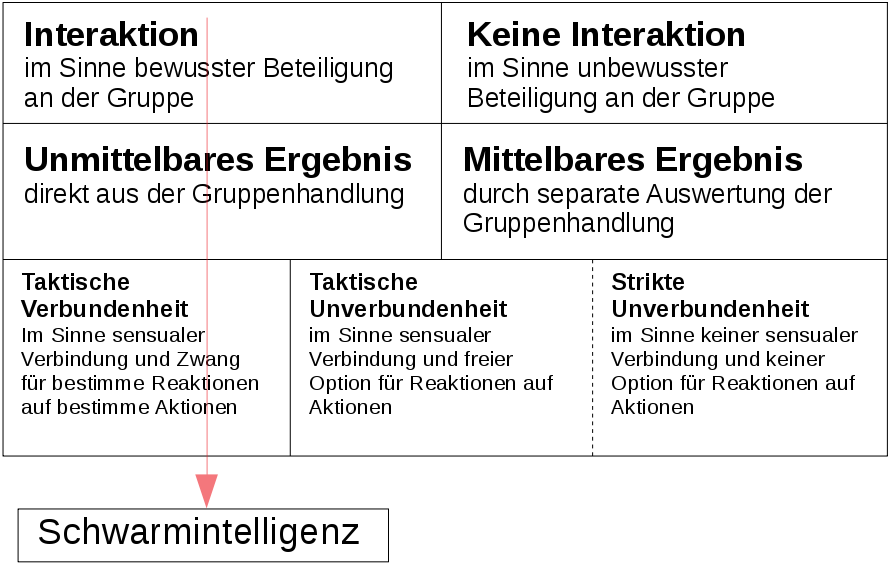
\includegraphics[width=1\textwidth]{schwarmintelligenz}
		\label{defabb}
	\end{center}
	\hspace{1in}\parbox{4in}{\caption[Entstehungsbedingungen und Definitionen kollektiver Intelligenz bei Tierschwärmen]{Entstehungsbedingungen und Definitionen kollektiver Intelligenz bei Tierschwärmen\footnotemark}}
\end{figure}
\footnotetext{A. Aulinger (2013)}
\begin{itemize}
	\item \textbf{Interaktion:} Auf Aktion und Reaktion basierende Interaktion gilt als Grundlage bzw. Rahmenbedingung für die Definition des Begriffs Schwarmintelligenz. Anlass dafür ist der in den Tieren vorhandene Instinkt, der diese veranlasst, sich bewusst an der Gruppe zu beteiligen.
	\item \textbf{Unmittelbares Ergebnis:} Einzelne Tiere führen Handlungen aus ohne Wissen um das Schwarmergebnis. Das Resultat entsteht unmittelbar aus der Handlung des Schwarms und bedarf keiner externen Aggregation und Auswertung.
	\item \textbf{Taktische Verbundenheit:} Sowohl die sensuale Verbindung der Tiere als auch der in den Tieren verankerte Instinkt zeugen von der taktischen Verbundenheit des Schwarms bestehend aus festen Aktions- und Reaktionsmustern. 
\end{itemize}
\par Zusammenfassend beschreibt der Begriff Schwarmintelligenz ein Phänomen aus dem Tierreich zur Selbstorganisation eines Schwarms, um lebensnotwendige Aufgaben gemeinsam und auf intelligente Weise zu bewältigen. Dabei vollbringen die Tiere im Schwarm Leistungen, die das Vermögen jedes Einzeltiers übersteigen.
\subsubsection{Ameisen}
Ein Ameisenstaat vollbringt Erstaunliches und passt sich ständig an neue Gegebenheiten seiner Umwelt an. Ameisen bilden Staaten mit einigen hundert bis zu mehreren Millionen Individuen. Trotz dieser riesigen Anzahl funktioniert ein Ameisenstaat, da er sich selbst organisiert ohne eine hierarchische Instanz, die einen Überblick über alle Aufgaben besitzt oder diese steuert und verteilt. Stattdessen führen die Handlungen einzelner Ameisen im Zusammenspiel zu einem organisierten Staat, der für die Ameisen sorgt und Nahrung, Brutpflege und Schutz bietet. Für die Informatik besonders interessant sind die Ameisen aufgrund ihrer Fähigkeit effiziente Wege zwischen Futterquellen und dem Ameisenbau ausfindig zu machen\footnote{L. Pintscher (2008)}.
\par Ist der Futtervorrat des Ameisenbaus erschöpft verlassen mehrere Ameisen den Ameisenbau gleichzeitig und begeben sich auf Futtersuche. Sobald eine Ameise eine Futterquelle gefunden hat, nimmt sie eine Gewichtseinheit des Futters mit und begibt sich auf den Rückweg zum Ameisenbau. Dabei setzt die Ameise Pheromone frei die mit der Zeit verfliegen, um den Weg zur Futterquelle zu markieren. Die Ameise die den kürzesten Weg zu einer Futterquelle gefunden hat legt die Strecke zwischen Ameisenbau und Futterquelle häufiger zurück.  Die Pheromonspur wird durch das häufige Zurücklegen der Strecke intensiviert und dient als sicherer Wegweiser zur Futterquelle. Mitglieder der Kolonie folgen den intensivsten Pheromonspuren. Ist die Futterquelle erschöpft, löst sich die Pheromonspur auf\footnote{R. Wehner (2001)}.
\subsubsection{Bienen}
Um den Gesamtenergiebedarf des Schwarms zu ermitteln, orientiert sich die einzelne Sammlerin an der Wartezeit bei der Übergabe des gesammelten Nektars an die Bienen die den Nektar speichern: Je voller die Futterspeicher, desto länger müssen die Speicherbienen nach leeren Zellen suchen. Je leerer die Speicher, desto schneller wird die Abgabe des Nektars abgewickelt.
\par Im kilometerweiten Gelände besitzt keine Biene den gesamten geographischen Überblick. Sie entscheidet nur lokal über die Rentabilität der Futterquelle. Kundschafterinnen und Sammlerinnen, die von der Futtersuche wiederkehren, führen einen Tanz auf und zeigen unbeschäftigten Bienen damit die Richtung und Entfernung zur Futterquelle. Unbeschäftigte Bienen sehen sich die Tänze der im Bienenstock eintreffenden Bienen an und entscheiden sich anschließend für ihr nächstes Ziel. Sobald eine Futterquelle erschöpft ist brauchen die Sammlerinnen länger beim Sammeln und veranlassen aufgrund der geringeren Anzahl an Tänzen weniger Bienen dazu am gleichen Ort zu sammeln.
\newpage
\subsection{Agentenbasierte Modellierung}
Die Agentenbasierte Modellierung erlaubt eine natürliche Beschreibung von Systemen als eine Sammlung autonomer entscheidungsfähiger Agenten in einer gemeinsamen Umgebung, um emergente Phänomene zu analysieren. Das Ziel der Agentenbasierten Modellierung besteht darin, durch die Simulation einer Vielzahl an Agenten, das resultierende Systemverhalten zu untersuchen. Nach C. Macal und M. North\footnote{C. Macal, M. North (2010)} verfügt ein agentenbasiertes Modell über folgende Komponenten:
\begin{itemize}
	\item \textbf{Agenten:} Agenten handeln autonom, proaktiv und reaktionär auf der Basis von festgelegten Regeln. Jeder Agent besitzt nur eine eingeschränkte Sicht auf das Gesamtsystem. Sein Wissen über den globalen Zustand des Systems ist immer unvollständig.
	\item \textbf{Agenten-Beziehungen:} Beziehungen zwischen Agenten entstehen durch die proaktive Aktion eines Agenten und die darauffolgende Reaktion eines anderen Agenten oder Interaktionen der Agenten mit der Umgebung.
	\item \textbf{Agenten-Umgebung:} Agenten interagieren innerhalb einer Umgebung mit anderen Agenten und ihrer Umgebung.
\end{itemize}
\subsubsection{Agenten} 
M. Wooldridge und N. Jennings\footnote{M. Wooldridge, N. Jennings (1995)} weisen Agenten die Charaktereigenschaften Autonomie, Proaktivität, Reaktivität und die Fähigkeit zur Interaktion durch Kommunikation zu. Die Handlungsautonomie eines Agenten beschränkt sich auf die Fähigkeit, eigenständig zu entscheiden, welche der ihm zur Verfügung stehenden Aktionen situationsbedingt auszuführen ist. Zielvorgaben bestimmen wann ein Agent welche Aktionen ausführt. Proaktivität beschreibt dabei das zielgerichtete Verhalten eines Agenten der selbst aktiv wird, statt nur auf die Umgebung zu reagieren.\newline
\subsubsection{Agenten-Beziehungen}
Zwischen den Systemelementen bestehen Interaktionsbeziehungen. Die technischen Voraussetzungen für die Kommunikation werden von der Umgebung bereitgestellt. Beziehungen lassen sich einteilen in Interaktion zwischen Agenten und Umgebung, Interaktion zwischen Agenten und organisatorisch bedingte Beziehungen. Die Kommunikation zwischen Agenten kann dabei direkt durch Austausch von Nachrichten oder indirekt über die Veränderung der Umgebung erfolgen.\newline
\subsubsection{Agenten-Umgebung}
Nach S. Russell und P. Norvig\footnote{S. Russel, P. Norvig (1995)} muss eine geeignete Agenten-Umgebung zugänglich, deterministisch, dynamisch, kontrollierbar und teleologisch sein. Eine zugängliche Umgebung erlaubt den Agenten Zugriff auf ihren Zustand. In der Regel beschränkt sich dieser Zugriff jedoch auf den lokalen Wahrnehmungsbereich eines Agenten und erlaubt somit nur Zugriff auf einen Ausschnitt der Umgebung. Deterministisch ist die Umgebung, sobald der Folgezustand vollständig durch den aktuellen Umgebungszustand und die aktuelle Aktion des Agenten bestimmt ist. Kann sich der Zustand der Umgebung durch Aktionen der Agenten ändern, so handelt es sich um eine dynamische und kontrollierbare Umgebung.
\newpage
\section{Schwarmintelligente Algorithmen}

\subsection{Particle Swarm Optimization}
Die klassische \ac{PSO} wurde erstmals im Jahr 1995 von J. Kennedy und R. Ebert beschrieben. Die \acs{PSO} stellt ein, auf der Abfolge von abstrakten Schritten basiertes, Verfahren zur näherungsweisen Lösung von Optimierungsproblemen dar. Zur Lösung des Optimierungsproblems wird eine Population von Partikeln, so lange durch einen Suchraum bewegt, bis eine hinreichende Lösung in einer angemessenen Zeit gefunden wird. Dabei stellt die Position eines Partikels eine potentielle Lösung dar und wird in jedem Zeitschritt neu berechnet. Um die \acs{PSO} auf ein mathematisches Problem anwenden zu können, muss zunächst der Suchraum und die Partikel definiert werden.
\subsubsection{Suchraum}
Der Suchraum $S \subset \mathbb{R}^n$ ist ein n-dimensionaler Raum, in dem sich die gesamte Population $X=\{x_{1},x_{2},...,x_{n}\}$ der Partikel bewegt. Damit eine Lösung gefunden werden kann beschränkt sich der Suchraum auf eine endliche Anzahl an möglichen Positionen, die von den Partikeln besucht werden können.
\subsubsection{Partikel}
Jedes Partikel $x_{i}$ besitzt dabei folgende Eigenschaften im Suchraum $S$ zum Zeitpunkt $t$:
\begin{itemize}
	\item Position $x_{i}(t)$ im Suchraum $S$ mit einem Funktionswert $f(x_{i}(t))$: Die aktuelle Position des Partikels $x_{i}$ zum Zeitpunkt $t$ repräsentiert eine potentielle Lösung des Optimierungsproblems. Der dazugehörende Funktionswert $f(x_{i}(t))$ beschreibt die Güte der potentiellen Lösung.
	\item Position $x_{b,i}(t)$ im Suchraum $S$ mit einem Funktionswert $f(x_{b,i}(t))$: Die Position $x_{b,i}$ ist die bisher beste Position des Partikels $x_{i}$ zum Zeitpunkt $t$.
	\item Position $x_{g}(t)$ im Suchraum $S$ mit einem Funktionswert $f(x_{g}(t))$: Die Position $x_{g}$ ist die bisher beste Position des Partikelschwarms zum Zeitpunkt $t$.
	\item Geschwindigkeit $v_{i}(t)$: Die Geschwindkeit $v_{i}$ mit der sich der Partikel durch den Suchraum $S$ zum Zeitpunkt $t$ bewegt.
	\item Trägheitskoeffizient $w$: Der Trägheitskoeffizient $w$ bestimmt die Gewichtung der Geschwindigkeit $v_{i}(t)$ zum Zeitpunkt $t+1$.
	\item lokaler Vertrauenskoeffizient $a_{l}$: Der lokale Vertrauenskoeffizient $a_{l}$ bestimmt die Gewichtung der lokalen Attraktion, bei der Berechnung der Geschwindigkeit $v_{i}(t+1)$.
	\item globaler Vertrauenskoeffizient $a_{g}$: Der globale Vertrauenskoeffizient $a_{g}$ bestimmt die Gewichtung der globalen Attraktion, bei der Berechnung der Geschwindigkeit $v_{i}(t+1)$.
\end{itemize}
Der Trägheitskoeffizient $w$ und die Vertrauenskoeffizienten $a_{l}$ und $a_{g}$ geben an, wie sehr die Partikel sich selbst, ihren eigenen Erfahrungen und den Erfahrungen ihrer Nachbarn vertrauen.
\newpage
\subsubsection{Algorithmus}
\begin{framed}
	\begin{algorithm}[H]
		Initialisiere Partikelschwarm $X$ im Suchraum $S$\;
		\While{Maximale Iterationen nicht erreicht}{
			Bestimme für jeden Partikel Position $x_{i}(t)$\;
			Berechne für jeden Partikel den Funktionswert $f(x_{i}(t))$\;
			\lIf{$f(x_{i}(t))$ besser als $f(x_{b,i}(t))$)}{
				Setze $x_{b,i}(t)$ = $x_{i}(t)$
			}
			\lIf{$f(x_{i}(t))$ besser als $f(x_{g}(t))$}{
				Setze $x_{g}(t))$ = $x_{i}(t)$
			}
			Berechne Geschwindigkeit vi(t) des Partikels xi\;
			Berechne neue Position xi(t+1) des Partikels xi\;
		}
		\caption{PSO Algorithmus}
		\label{psoalgo}
	\end{algorithm}
\end{framed}
Der abgebildete Algorithmus zeigt den Ablauf der klassischen \acs{PSO} anhand von Pseudocode. Im ersten Schritt wird die Population $X$ mit zufälligen Positionen $x_{i}$ im Suchraum $S$ initialisiert. Bis die Anzahl an maximalen Iterationen nicht erreicht ist wird für jeden Partikel geprüft ob der Funktionswert $f(x_{i}(t))$ für die Position $x_{i}$ besser ist als der Funktionswert $f(x_{i}(t-1))$ im vorherigen Schritt an der Position $x_{i}(t-1)$. Ist der Funktionswert $f(x_{i}(t))$ für die Position $x-{i}(t)$ des Partikels besser, wird die bisher beste Position des Partikels $x_{b,i}(t)$ zu $x_{i}(t)$. Zudem wird für jeden Partikel $x_{i}$ geprüft, ob der aktuelle Funktionswert $f(x_{i}(t))$ des Partikels besser ist als der globale Funktionswert $f(x_{g}(t))$. Ist dies der Fall so wird die global beste Position $x_{g}(t) zu x_{i}(t)$. Aus diesem Grund wurden in Weiterentwicklungen des Algorithmus Nachbarschaftsbeziehungen entwickelt. Es gibt viele Möglichkeiten die Nachbarschaftsbeziehungen zu realisieren. Im Rahmen dieser Studienarbeit wird darauf verzichtet. Für die nächste Iteration wird die Geschwindigkeit $v_{i}(t+1)$ und die neue Position $x_{i}(t+1)$ des Partikels nach folgenden Formeln berechnet:
\begin{eqnarray}
v_{i}(t+1) = wv_{i}(t) + a_{l}r_{1}(x_{b,i}(t) - x_{i}(t)) + a_{g}r_{2}(x_{g}(t) - x_{i}(t)) \\
x_{i}(t+1) = x_{i}(t) + v_{i}(t+1)
\end{eqnarray}
\par Bei der Berechnung der neuen Geschwindigkeit $v_{i}(t+1)$ wird die Entfernung der Position  $x_{g}(t)$ zur Position $x_{b,i}(t)$ berechnet. Dabei fallen die Zufallszahlen $r_{1}$, $r_{2} \subset \subset \mathbb{R}$ ins Gewicht, sowie die Konstanten $w$, $a_{l}$, $a_{g}$, mit denen das Verhalten des Schwarms verändert wird. Gilt $a_{l} > a_{g}$, dann streben die Partikel in Richtung von $x_{b,i}(t)$. Ist $a_{g} > a_{l}$, dann konvergieren die Partikel zur Position $x_{g}(t)$. Abbildung 2 zeigt in grafischer Darstellung die Berechnung der neuen Geschwindigkeit $v_{i}(t+1)$ und der neuen Position $x_{i}(t+1)$.
\begin{figure}[h]
	\begin{center}
		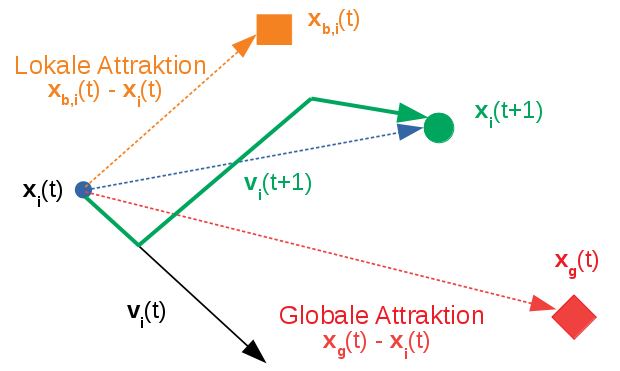
\includegraphics[width=0.55\textwidth]{pso}
	\end{center}
	\hspace{1in}\parbox{4in}{\caption[Berechnung von $x_{i}(t+1)$ und $v_{i}(t+1)$]{Berechnung von $x_{i}(t+1)$ und $v_{i}(t+1)$}}
	\label{psoabb}
\end{figure}
\subsection{Ant Colony Optimization}

\subsection{Bee Colony Optimization}
\section{Modellplanung und Framework}
\section{Implementierung}
\section{Zusammenfassung}

\newpage
\begin{thebibliography}{sotief}
	\bibitem{1}W.M. Wheeler. The Ant Colony as an Organism. Journal of Morphology Volume 22, Issue 2, Seite 307-325. Entstehungsjahr: 1911.\newline\newline Weblink:
	http://www3.interscience.wiley.com/journal/109914213/abstract. . Einsichtnahme: 25.02.2018
\end{thebibliography}
\newpage
%\appendix
\appendixtoc
\newpage
\section{Anhang 1} 
\end{document}


